% zip files.zip ms63.tex CMD_cuts_double.pdf main_figure.pdf gap.pdf vb_vs_teff.pdf vb_vz.pdf field_comparison.pdf bib.bib ms.pdf

\documentclass{aastex63}

% Latin
\newcommand{\ie}{{\it i.e.}}
\newcommand{\eg}{{\it e.g.}}
\newcommand{\etal}{{\it et al.}}

% Missions & Spacecraft
\newcommand{\kepler}{{\it Kepler}}
\newcommand{\Kepler}{{\it Kepler}}
\newcommand{\corot}{{\it CoRoT}}
\newcommand{\Ktwo}{{\it K2}}
\newcommand{\ktwo}{\Ktwo}
\newcommand{\TESS}{{\it TESS}}
\newcommand{\tess}{{\it TESS}}
\newcommand{\LSST}{{\it LSST}}
\newcommand{\lsst}{{\it LSST}}
\newcommand{\Wfirst}{{\it WFIRST}}
\newcommand{\wfirst}{{\it WFIRST}}
\newcommand{\SDSS}{{\it SDSS}}
\newcommand{\PLATO}{{\it PLATO}}
\newcommand{\plato}{{\it PLATO}}
\newcommand{\Gaia}{{\it Gaia}}
\newcommand{\gaia}{{\it Gaia}}
\newcommand{\panstarrs}{{\it PanSTARRS}}
\newcommand{\LAMOST}{{\it LAMOST}}

% Units and Quantities
\newcommand{\Teff}{$T_{\mathrm{eff}}$}
\newcommand{\teff}{$T_{\mathrm{eff}}$}
\newcommand{\FeH}{[Fe/H]}
\newcommand{\feh}{[Fe/H]}
\newcommand{\prot}{$P_{\mathrm{rot}}$}
\newcommand{\pmega}{$\bar{\omega}$}
\newcommand{\logg}{log(g)}
\newcommand{\dnu}{$\Delta \nu$}
\newcommand{\numax}{$\nu_{\mathrm{max}}$}
\newcommand{\degrees}{$^\circ$}
\newcommand{\vx}{$v_{\bf x}$}
\newcommand{\vy}{$v_{\bf y}$}
\newcommand{\vz}{$v_{\bf z}$}
\newcommand{\vb}{$v_{\bf b}$}
\newcommand{\kms}{kms$^{-1}$}
\newcommand{\sigmavb}{$\sigma_{v{\bf b}}$}
\newcommand{\sigmavz}{$\sigma_{v{\bf z}}$}

% Paper-specific and other
\newcommand{\mura}{$\mu_\alpha$}
\newcommand{\mudec}{$\mu_\delta$}
\newcommand{\parallax}{$\pi$}
\newcommand{\gcolor}{$G_{BP} - G_{RP}$}
\newcommand{\mcp}{\citep{mcquillan2014}}
\newcommand{\mct}{\citet{mcquillan2014}}
\newcommand{\bvector}{${\bf b}$}
\newcommand{\python}{{\it Python}}
\newcommand{\racomment}[1]{{\color{blue}#1}}

% \shorttitle{Calibrating gyrochronology with kinematics}
% \shortauthors{Angus \etal}

\begin{document}

\title{Calibrating gyrochronology using Galactic kinematics}

% \correspondingauthor{Ruth Angus}
% \email{rangus@amnh.org}

\author{Ruth Angus}
\affiliation{Department of Astrophysics, American Museum of Natural History,
200 Central Park West, Manhattan, NY, USA}
\affiliation{Center for Computational Astrophysics, Flatiron Institute,
162 5th Avenue, Manhattan, NY, USA}
\affiliation{Department of Astronomy, Columbia University, Manhattan, NY, USA}

\author{Yuxi (Lucy) Lu}
\affiliation{Department of Astronomy, Columbia University, Manhattan, NY, USA}
\affiliation{Department of Astrophysics, American Museum of Natural History,
200 Central Park West, Manhattan, NY, USA}

\author{Dan Foreman-Mackey}
\affiliation{Center for Computational Astrophysics, Flatiron Institute,
162 5th Avenue, Manhattan, NY, USA}

\author{Adrian M. Price-Whelan}
\affiliation{Center for Computational Astrophysics, Flatiron Institute,
162 5th Avenue, Manhattan, NY, USA}

\author{Jason Curtis}
\affiliation{Department of Astrophysics, American Museum of Natural History,
200 Central Park West, Manhattan, NY, USA}

\author{Emily Cunningham}
\affiliation{Center for Computational Astrophysics, Flatiron Institute,
162 5th Avenue, Manhattan, NY, USA}

\begin{abstract}
Gyrochronology, the method of inferring the age of a star from its rotation
period, could provide ages for billions of stars over the coming decade of
time-domain astronomy.
However, the gyrochronology relations remain poorly calibrated due to a lack
of precise ages for old, cool main-sequence stars.
Now however, with proper motion measurements from Gaia, Galactic kinematics
can be used as an age proxy, and the magnetic and rotational evolution of
stars can be examined in detail.
We demonstrate that kinematic ages, inferred from the velocity dispersions of
groups of stars, beautifully illustrate the time and mass-dependence of the
gyrochronology relations.
We use the kinematic ages of field stars, plus benchmark clusters and
    asteroseismic stars, to calibrate a new empirical Gaussian process
    gyrochronology relation, that fully captures the complex rotational
    evolution of cool dwarfs over a range of masses and ages.
We use cross validation to demonstrate that this relation accurately predicts
ages for FGKM dwarfs.
\end{abstract}

\keywords{
Stellar Rotation ---
Stellar Evolution ---
Stellar Activity ---
Stellar Magnetic Fields ---
Low Mass Stars ---
Solar Analogs ---
Milky Way Dynamics
}

\section{Introduction}

% Motivation
Main-sequence dwarfs are the most common stars in the Milky Way, and their
ages could reveal the evolution of Galactic stellar populations and planetary
systems.
However, the ages of low-mass stars, particularly K and M dwarfs are difficult
to measure because their luminosities and temperatures evolve slowly on the
main sequence \citep[see][for a review of stellar ages]{soderblom2010}.
Fortunately, rotation-dating, or `gyrochronology’ provides a promising means
to measure precise ages for these cool dwarfs.
\citep[\eg][]{schatzman1962, weber1967, kraft1967, skumanich1972, kawaler1988,
pinsonneault1989, barnes2003, barnes2007, mamajek2008, barnes2010, meibom2011,
epstein2014, meibom2015, vansaders2016, vansaders2018, claytor2020}.
The rotation periods of GKM stars evolve relatively rapidly, and a fully
calibrated gyrochronology model that captures the time and mass-dependence of
stellar spin down could provide ages that are precise to within 20\% for
millions of Milky Way stars in the time-domain era \citep{epstein2014,
najita2016, angus2019, claytor2020}.
However, gyrochronology models are not yet fully calibrated, especially for
K and M dwarfs.
% What do we still not understand?
% Gyro is still poorly calibrated
% With the thousands of new photometric rotation period measurements provided by
% specialized ground and space-based missions \citep[particularly \kepler/\ktwo\
% and \tess][]{borucki2010, howell2014, ricker2015}, we are making progress
% towards the ultimate goal for rotation-dating: a fully calibrated
% gyrochronology relation that is applicable to GKM main-sequence stars of all
% ages.
A lack of suitable low-mass and old calibration stars limits the reliable mass
and age coverage of gyrochronology relations.
For example, the oldest K dwarfs in an open cluster (and therefore having a
precise age estimate), with measured rotation periods, are those in Ruprecht
147 (2.7 Gyr) \citep{curtis2020, age_citation}.
The oldest cluster M dwarfs with measured rotation periods are those in
Praesepe (600-700 Myr) \citep{douglas2017, rebull2017, age_citation}.
Gyrochronology relations can therefore be considered untested for K dwarfs
older than 2.7 Gyr and M dwarfs older than 600-700 Myr.

Historically, gyrochronology calibration samples have mainly been comprised of
stars in open clusters and stars with detectable acoustic pulsations, both of
which can be precisely dated with stellar evolution models.
The rotation periods of these calibration stars can often be measured with
precise time-series photometry, and the Kepler spacecraft has played a leading
role in providing light curves for stellar rotation studies
\citep[\eg][]{borucki2010, meibom2011, mcquillan2013, mcquillan2014,
howell2014, reinhold2014, garcia2014, aigrain2015, meibom2015, douglas2016,
douglas2017, rebull2016, rebull2017, santos2019, reinhold2019, rebull2020,
gordon2020, curtis2020, breton2021}.
Magnetically active regions on the surfaces of stars create dark and bright
surface features which produce periodic variability in the overall brightness
of a rotating star.
This variability is, at most, on the order of 1\% of the star's overall flux.
The rotation periods of stars can often be measured from their light curves
using signal-processing techniques.
TESS, the Transiting Exoplanet Survey Satellite, is continuing the legacy of
Kepler and will provide rotation periods for many more stars
\citep{ricker2014}.

% For the purposes of calibrating gyrochronology, open clusters provide good
% mass coverage for young stars: rotation periods have been measured for F to
% mid M dwarfs up to ages of around 700 Myr.
% In contrast, asteroseismic stars provide reasonable age coverage for hot
% stars: ages and photometric surface rotation periods have been measured for F,
% G and early K dwarfs up to ages of 10 Gyr.
% However, neither asteroseismology nor cluster analysis can provide rotation
% periods and ages for old, late K and M dwarfs.
% In addition, cluster and asteroseismic stars generally provide sparse coverage
% of the rotation period-effective temperature plane, and cannot reveal the
% detailed evolution of stellar rotation rates.
% As a result, most empirical gyrochronology relations are only reliable for G
% dwarfs up to Solar age, K dwarfs up to 2-3 Gyr, and early M dwarfs up to $<$ 1
% Gyr.

To extend gyrochronology relations to older K and M dwarfs, it may be
necessary to use alternative dating methods.
Old open clusters are generally too distant for photometric rotation period
measurements of faint M dwarfs, and asteroseismic analyses suffer from the
large magnetic activity signals and low-amplitudes of oscillations for
low-mass stars.
There is great promise, however, for binary studies as an alternative method
for calibrating gyrochronology.
For example, low-mass K and M dwarfs with a precisely dateable co-moving
companion (\eg\ a white dwarf, a subgiant, or a star with detectable acoustic
oscillations) could be good calibrators.
We have recently investigated the promise of kinematics as an alternative
age-dating method.
In \citet{angus2020} we explored the kinematic properties of Kepler field
stars with measured rotation periods and found that the velocity dispersion of
stars increase with stellar rotation period, as expected.
In \citet{lu2021} we used the velocity dispersions of Kepler field stars to
estimate their ages using an Age-Velocity dispersion Relation (AVR).
In this work, we use these kinematic ages for around 30,000 Kepler field
stars to extend the gyrochronology relations into the old K and early M dwarf
regime.

% % Gyro 101
% Stars with significant convective envelopes ($\lesssim$ 1.3 M$_\odot$) have
% strong magnetic fields which are thought to be generated by a Solar-type
% $\alpha-\Omega$ dynamo.
% These stars lose angular momentum over long timescales via magnetic braking
% \citep[\eg][]{schatzman1962, weber1967, kraft1967, skumanich1972, kawaler1988,
% pinsonneault1989}.
% Stars arrive on the main sequence with a random distribution of rotation
% periods, ranging from 1 oto 10 days \citep{rebull2019}, however the rotation
% periods of stars in open clusters have converged onto a unique age-rotation
% period-mass sequence by $\sim$500-700 million years \citep[\eg][]{irwin2009,
% gallet2013}.
% After this time, the rotation period of a star is thought to be determined, to
% first order, by its photometric color/effective temperature/mass and age
% \citep[\eg]{barnes2003, barnes2007, barnes2010, meibom2011, meibom2015}.

% The rate at which a star loses angular momentum is thought to chiefly depend
% on its magnetic field strength.
% Lower-mass stars with deeper convection zones have stronger magnetic fields,
% thus larger Alfvén radii, and therefore experience greater angular momentum
% loss rates \citep[\eg][]{schatzman1962, kraft1967, parker1970, kawaler1988,
% charbonneau2010}.
% This effect dominates the evolutionary sequence of young stars and, for
% example in the $\sim$ 700 Myr Praesepe cluster, rotation rate increases with
% increasing mass (rotation {\it period decreases} with increasing mass).
% However, at ages greater than around 1 Gyr \citep{spada2019, curtis2019,
% angus2020}, internal angular momentum transport becomes important and starts
% to influence the evolution of surface rotation periods.

% % Core-envelope coupling
% A period of core-envelope decoupling is necessary to explain the observed
% rotation periods of stars in extremely young open clusters (1-10 Gyr)
% \citep[\eg][]{irwin2007, bouvier2008, denissenkov2010, spada2011, reiners2012,
% gallet2013}.
% After the development of a radiative core, little angular momentum is
% transported between the core and convective envelope and, if wind-braking
% slows the surface substantially before the two zones recouple, the core may
% rotate much more quickly than the envelope.
% The Sun rotates almost as a solid body \citep[\eg][]{thompson1996}, so it is
% expected that the cores and envelopes of Solar-like stars eventually
% re-couple, with angular momentum efficiently transported between them.
% The timescales for recoupling have been studied extensively and explored in
% theoretical models for decades \citep[\eg][]{endal1981, macgregor1991,
% denissenkov2010, gallet2013, lanzafame2015}.
% The physical mechanism responsible for internal angular transport is still
% unknown, however magnetic field-induced coupling and gravity waves are two
% processes often used to explain the phenomenon \citep[see,
% \eg][]{charbonneau1993, ruediger1996, spruit2002, talon2003, spada2010,
% brun2011, oglethorpe2013}.
% Based on observations of lithium depletion and rotation period evolution in
% open clusters, including new rotation period measurements for the $\sim$1 Gyr
% NGC6811 cluster \citep{curtis2019}, the coupling timescale has been determined
% to be strongly mass-dependent \citep{lanzafame2015, somers2016, spada2019}.
% Semi-empirical models with mass-dependent angular momentum transport are able
% to reproduce the rotation periods in open clusters and the field
% \citep{spada2019, angus2020}.

\subsection{Core-envelope decoupling}

% Describe previous paper
In Angus \etal\ (2020) we demonstrated that Galactic kinematics can be used to
explore the evolution of stellar rotation.
We showed that velocity dispersion, an established age proxy in the Galactic
thin disk, increases smoothly as a function of rotation period, indicating
that rotation period increases with age as expected.
Using velocity dispersion as an age proxy, we also showed that old K dwarfs
spin down more slowly than G dwarfs: their rotational evolution appears to
`stall' after around 1 Gyr, in a manner that reflects the behavior of K dwarfs
observed in open clusters \citep{curtis2019}.
At young ages ($\sim$ 0.5 -- 1 Gyr), K dwarfs spin more slowly than G dwarfs of
the same age, because their deeper convection zones generate stronger magnetic
fields, which leads to more efficient magnetic braking.
However, at old ages ($\gtrsim$ 1 Gyr) K dwarfs rotate at the same rate or
more rapidly than contemporary G dwarfs.
The leading explanation for this phenomenon is that angular momentum is
transferred from the core to the surface over longer timescales for lower-mass
stars \citep{spada2019}, \ie\ they experience a more extended phase of
`core-envelope decoupling'.

% The angular momentum of the radiative cores and convective envelopes of stars
% are thought to evolve separately at young ages \citep[\eg][]{mcdonald1995,
% gallet2013}.
A period of core-envelope decoupling is necessary to explain the observed
rotation periods of stars in extremely young open clusters (1-10 Gyr)
\citep[\eg][]{irwin2007, bouvier2008, denissenkov2010, spada2011, reiners2012,
gallet2013}.
During this phase there is little transfer of angular momentum between
radiative core and convective envelope and, as wind-braking removes angular
momentum from the envelope, it decelerates while the core continues to spin
rapidly.
Over time however, angular momentum is transported across the interface
between the two zones, and momentum from the rapidly spinning interior
surfaces, inhibiting the deceleration of the outer envelope.
% With a mass-dependent timescale for core-envelope coupling semi-empirical
% models are able to reproduce the
Currently, the rotation periods of field and cluster stars can only be
reproduced by semi-empirical models with a mass-dependent timescale for
core-envelope coupling \citep[][Angus \etal, 2020]{spada2019, curtis2019}.


% Summary of using velocity dispersions as an age proxy -- lit review
\subsection{Using kinematics as an age proxy}

The star forming molecular gas clouds observed in the Milky Way have a low
out-of-plane, or vertical, velocity \citep[\eg][]{stark1989, stark2005,
aumer2009, martig2014, aumer2016}.
In contrast, the vertical velocities of older stars are observed to be larger
in magnitude on average \citep{stromberg1946, wielen1977, nordstrom2004,
holmberg2007, holmberg2009, aumer2009, casagrande2011, ting2019, yu2018}.
There are two possible explanations for this observed increase in velocity
dispersion with age: either stars are born kinematically `cool' and their
orbits are heated over time via interactions with giant molecular clouds
\citep[see][for a review of secular evolution in the MW]{sellwood2014}, or
stars formed kinematically `hotter' in the past \citep[\eg][]{bird2013}.
Either way, the vertical velocity dispersions of thin disk stars are observed
to increase with stellar age.
This behavior is codified by Age-Velocity dispersion Relations (AVRs), which
typically express the relationship between age and velocity dispersion as a
power law: $\sigma_v \propto t^\beta$, with free parameter, $\beta$
\citep[\eg][]{holmberg2009, yu2018}.
These expressions can be used to infer the ages of groups of stars from their
velocity dispersions, as we do in this paper (see section \ref{sec:method}).

Kinematic ages have been used to explore the evolution of cool dwarfs for over
a decade.
\citet{west2004, west2006} found that the fraction of magnetically active M
dwarfs decreases over time, by using the vertical distances of stars from the
Galactic mid-plane as an age proxy, and \citet{west2008} used kinematic ages
to calculate the expected activity lifetime for M dwarfs of different spectral
types.
\citet{faherty2009} used tangential velocities to infer the ages of M, L and T
dwarfs, and showed that dwarfs with lower surface gravities tended to be
kinematically younger, and \citet{kiman2019} used velocity dispersion as an
age proxy to explore the evolution of H$\alpha$ equivalent width (a magnetic
activity indicator), in M dwarfs.

% After the development of a radiative core, little angular momentum is
% transported between the core and convective envelope and, if wind-braking
% slows the surface substantially before the two zones recouple, the core may
% rotate much more quickly than the envelope.
% The Sun rotates almost as a solid body \citep[\eg][]{thompson1996}, so it is
% expected that the cores and envelopes of Solar-like stars eventually
% re-couple, with angular momentum efficiently transported between them.
% The timescales for recoupling have been studied extensively and explored in
% theoretical models for decades \citep[\eg][]{endal1981, macgregor1991,
% denissenkov2010, gallet2013, lanzafame2015}.

AVRs are usually calibrated in Galactocentric velocity coordinates (\vx, \vy,
\vz\ or $UVW$), and these velocities can only be calculated with full 6D
positional and velocity information, however most \kepler\ rotators do not
have RV measurements\footnote{Although RVs for most will be released in \gaia\
DR3}.
In Angus \etal\ (2020) we used velocity in the direction of Galactic latitude
(\vb) as a stand-in for \vz\ because, in the {\it Galactic} coordinate system,
velocities can be calculated from 3D positions and {\it 2D} proper motions.
The \kepler\ field lies at low Galactic latitude, so \vb\ is a close
approximation to \vz.
Though \vb\ velocity dispersion does not equal \vz\ velocity dispersion, it
still increases monotonically over time and provides accurate age rankings for
\kepler\ stars.
Unfortunately however, given that AVRs are calibrated in {\it Galactocentric}
coordinates (\vx, \vy, \vz), we could not directly translate \vb\ velocity
dispersions to ages.

In this paper, our aim was to use kinematic ages to calibrate a new
gyrochronology relation, for which four main steps were required.
Firstly, we inferred {\it vertical} velocity, \vz, for each star without an RV
measurement by marginalizing over missing RVs using a hierarchical Bayesian
model (see section \ref{sec:velocity_inference}).
Secondly, we calculated velocity dispersion for every star using a moving, or
rolling dispersion method (see section \ref{sec:velocity_dispersion}).
Thirdly, these velocity dispersions were converted into ages using an AVR
\citep[][section \ref{sec:avr}]{yu2018}.
Finally, we used a Gaussian process model to capture the complexities of
stellar rotational evolution and calibrated a new gyrochronology relation
using our kinematic ages, plus benchmark cluster and asteroseismic stars in
section \ref{sec:gp_model}.


\section{Method}

\subsection{Data}
\label{sec:data}

This study focuses on stellar rotation in the original \kepler\ field.
This is partly because \kepler\ provides the largest sample of published,
homogeneously measured rotation periods, and partly because its low Galactic
latitude allows us to marginalize over missing RV measurements and approximate
vertical velocity, \vz.
We combined three rotation period catalogs constructed from original \kepler\
data: \citet{mcquillan2014}, \citet{santos2019} and \citet{garcia2014}.

\begin{figure}[ht!]
\caption{Vertical velocities calculated with full 6D information vs vertical
    velocities inferred without RV, for all 3000 \mct\ stars with \gaia\ RV
    measurements.}
  \centering
    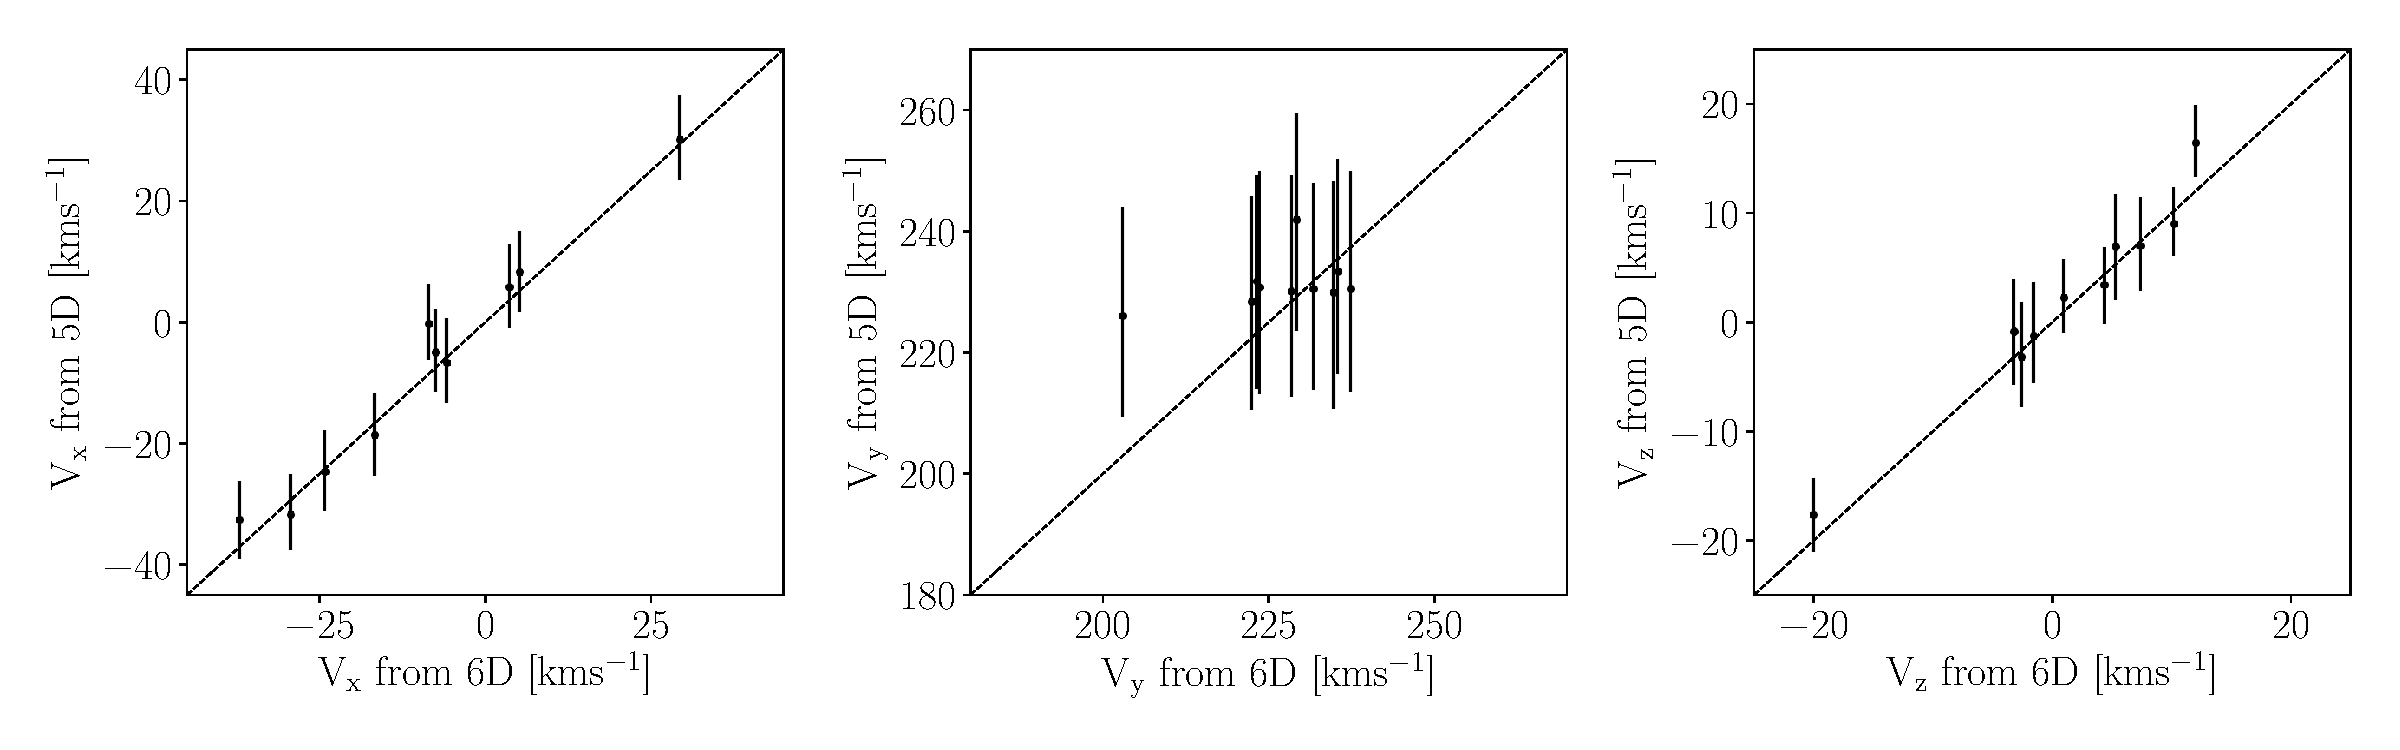
\includegraphics[width=1\textwidth]{v_comparison}
\label{fig:existing_rvs}
\end{figure}

\subsection{Inferring 3D velocities (marginalizing over missing RV
measurements)}
\label{sec:velocity_inference}

It has been demonstrated that the dispersion in vertical velocity, \vz\, for a
group of stars increases with the age of that group (citations).
However, velocities in Galactocentric coordinates, \vx, \vy\ and \vz, can only
be calculated with full 6-D position and velocity information, \ie\ proper
motions, position and radial velocity.
In Angus \etal\ (2020) we introduced the idea that kinematic ages could be
used to calibrate gyrochronology and showed, in the appendix of that paper,
that velocity, \vb\ in the Galactic frame, which can be calculated without an
RV measurement, can be used as an approximation to \vz\ for \kepler\ stars.
This is because the \kepler\ field of view lies at relatively low Galactic
latitudes, ($\sim 5-20$\degrees), so the $z$-direction is similar to the
$b$-direction for \kepler\ stars.
However, \vb\ is only a close approximation to \vz\ at extremely {\it low}
latitudes, and even in the \kepler\ field, kinematic ages calculated with \vb\
instead of \vz\ are systematically larger because of extra noise introduced by
the imperfect translation between \vb\ and \vz\.
In order to calculate accurate vertical velocities and therefore ages, the
appropriate approach is to {\it infer} \vz\  by marginalizing over missing RV
measurements.

Three-dimensional velocities in galactocentric coordinates: \vx, \vy, and \vz\
can only be directly computed via a transformation from 3D velocities in
another coordinate system, like the equatorial coordinates provided by \gaia:
\mura, \mudec, and RV.
For stars with no measured RV in \gaia\ DR2, \vx, vy, and \vz\ can still be
inferred from positions and proper motions alone, by marginalizing over
missing RV measurements.
For each star in our sample, we inferred \vx, \vy, and \vz\ from the 3D
positions and proper motions provided in the \gaia\ DR2 catalog
\citep{brown2011}.
We also simultaneously inferred distance, instead of using 1/\parallax, to
model velocities \citep{bailer-jones2015, bailer-jones2018}.

Using Bayes rule, the posterior probability of the parameters given the data
can be written:
\begin{equation}
p(v_{\bf xyz}, D | \mu_{\alpha}, \mu_{\delta}, \alpha, \delta, \pi) =
    p(\mu_{\alpha}, \mu_{\delta}, \alpha, \delta, \pi | v_{\bf xyz}, D)
    p(v_{\bf xyz}) p(D),
\end{equation}
where D is distance, $\alpha$ is Right Ascension (RA), $\delta$ is declination
(dec), $\pi$ is parallax, $\mu_\alpha$ is proper motion in RA, and
$\mu_\delta$ is proper motion in dec.
The prior over $\log$(distance) and velocities was a multivariate Gaussian
with mean and covariance determined from the distance and velocity
distributions of \kepler\ targets with RV measurements.

The posterior PDF was explored using {\tt emcee} \citep{foreman-mackey2013},
an affine-invariant, ensemble MCMC sampler.

Initialization.

We found that 10,000 samples with 16 walkers was sufficient to calculate a
converged autocorrelation time, and produce 150-500 independent samples per
parameter.

Over 3000 stars in the \mct\ sample do have RV measurements and provide an
opportunity to test this method of inferring velocities.
Figure \ref{fig:v_comparison} shows the velocities of these 3000 stars,
calculated using RV measurements, compared with their inferred velocities.

\begin{figure}[ht!]
\caption{Vertical velocities calculated with full 6D information vs vertical
    velocities inferred without RV, for all 3000 \mct\ stars with \gaia\ RV
    measurements.}
  \centering
    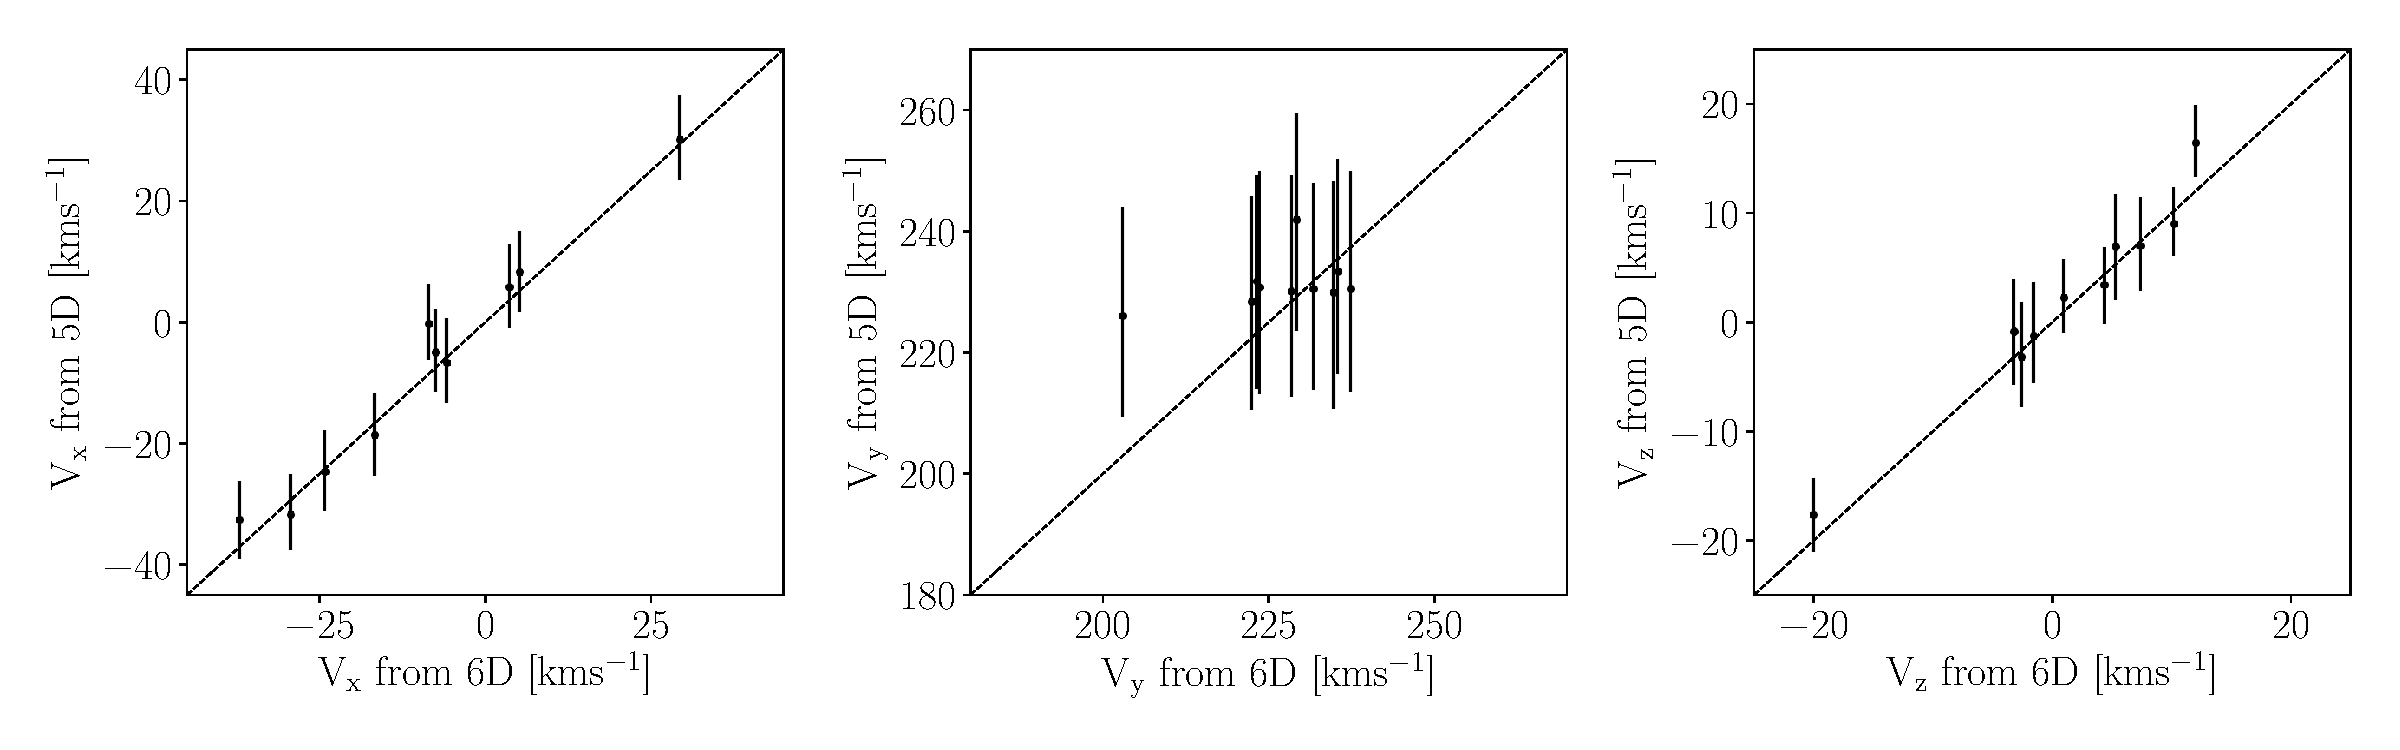
\includegraphics[width=1\textwidth]{v_comparison}
\label{fig:v_comparison}
\end{figure}

\subsection{Calculating velocity dispersions}
\label{sec:velocity_dispersion}

A kinematic age can be calculated from the velocity dispersion (\eg\ the
standard deviation or Median Absolute Deviation, MAD, of velocities) of a
group of stars.
These velocity dispersions can then be converted into an age using an AVR
\citep[\eg][]{holmberg2009, yu2018}.
The major assumption underlying kinematic ages is that all stars used to
calculate a velocity dispersion are {\it the same age}.
So, in order to calculate kinematic ages from velocity dispersions for
\kepler\ stars, it is necessary to group them by age.
Fortunately, we can use the implicit assumption that underpins gyrochronology
itself to group stars by age: that stars with the same rotation period and
color are the same age.
We discuss the implications of this assumption, and how our results would
change if this assumption is false, in the Discussion of this paper (section
\ref{sec:discussion}).

To calculate a \vz\ velocity dispersion and therefore age for each \kepler\
star, we grouped stars with their neighbors in
\logp--\teff\ space.
We experimented with two methods of grouping stars: using K-nearest neighbors,
and using a fixed range in \logp\ and \teff.
In the K-nearest neighbors method, each star was grouped with the K-nearest
stars in \logp-\teff\ space.
Groups created this way span a small range of \logp\ and \teff\ where the
number density of stars is large, and a large range where the number density
is small.
However, all groups have the same number of stars.
In the fixed range method, each star was grouped with stars whose \logp s and
\teff s fell within a certain range of their own.
This method created groups with large numbers of stars in densely populated
regions of the \logp--\teff\ plane, and small numbers of stars in sparsely
populated regions, \ie\ each group contains a different number of stars.
However, the bin size was constant.
To choose the best method, and to optimize for the parameters of each (K and
\logp\ and \teff-range), we conducted a set of tests.

\subsection{Converting velocity dispersion to age with an AVR}
\label{sec:avr}

\subsection{Comparing kinematic ages with asteroseismic and cluster ages}


\subsection{A Gaussian process gyrochronology relation}
\label{sec:gp_model}


\section{Results}

\subsection{A Gaussian process gyrochronology relation}
\label{sec:gp_model}

To calibrate a new gyrochronology relation, we fit a Gaussian process-based
model to the kinematic ages described above, as well as a set of field and
cluster benchmark stars.
These benchmark stars are stars with precise rotation periods measured from
Kepler/K2 light curves, and well-determined ages from cluster isochrone
fitting or asteroseismology.



\section{Discussion}


\section{Conclusion}

% Summarise motivation

% Summarise method

% Summarise results

% Summarise future


This work was partly developed at the 2019 KITP conference `Better stars,
better planets'.
Parts of this project are based on ideas explored at the Gaia sprints at the
Flatiron Institute in New York City, 2016 and MPIA, Heidelberg, 2017.
This work made use of the gaia-kepler.fun crossmatch database created by Megan
Bedell.

Some of the data presented in this paper were obtained from the Mikulski
Archive for Space Telescopes (MAST).
STScI is operated by the Association of Universities for Research in
Astronomy, Inc., under NASA contract NAS5-26555.
Support for MAST for non-HST data is provided by the NASA Office of Space
Science via grant NNX09AF08G and by other grants and contracts.
This paper includes data collected by the Kepler mission. Funding for the
\Kepler\ mission is provided by the NASA Science Mission directorate.

This work has made use of data from the European Space Agency (ESA) mission
{\it Gaia} (\url{https://www.cosmos.esa.int/gaia}), processed by the {\it
Gaia} Data Processing and Analysis Consortium (DPAC,
\url{https://www.cosmos.esa.int/web/gaia/dpac/consortium}).
Funding for the DPAC has been provided by national institutions, in particular
the institutions participating in the {\it Gaia} Multilateral Agreement.


\bibliography{bib}{}
\bibliographystyle{aasjournal}

\end{document}
